%%%%%%%%%%%%%%%%%%%%%%%%%%%%%%%%%%%%%%%%%%%%%%%%%%%%%%%%%%%%%%%%%%%%%%%%%%%%%%%
%     enunciado.tex:    Enunciado de la pr�ctica 2 de GIEAI-Inform�tica
%%%%%%%%%%%%%%%%%%%%%%%%%%%%%%%%%%%%%%%%%%%%%%%%%%%%%%%%%%%%%%%%%%%%%%%%%%%%%%%

\documentclass[english,a4paper,11pt]{article}

\usepackage[latin1]{inputenc}  % codificaci�n de caracteres de este archivo
\usepackage[spanish]{babel}    % Traducir: ``abstract'' ---> ``resumen''   etc.
\usepackage{fancyhdr}          % p�ginas con cabecera y pie
\usepackage{listings}          % listados de c�digo fuente
\usepackage{float}             % para que los listados floten como las figuras
\usepackage{vmargin}           % ajuste de m�rgenes f�cil de usar
\usepackage[T1]{fontenc}       % meter fuentes vectoriales
\usepackage{graphicx}          % figuras
\usepackage{upquote}           % comilla recta con \textquotesingle
\usepackage{placeins}          % orden \FloatBarrier para mantener figuras a raya

\usepackage[implicit=false]{hyperref}  % enlaces web (el par�metro implicit=false
                                       % evita problemas con el # de #include etc.)
                                       % uso expl�cito: \href[options]{URL}{text}
                                       %                \url{URL}

% mis abreviaturas
\newcommand{\C}{\texttt{C}}            % escribir� \C en lugar de \texttt{C}
\newcommand{\Pascal}{\texttt{Pascal}}  % idem con \Pascal ...
\newcommand{\fun}[1]{\texttt{#1()}}    % "\fun{main}" ---> "main()" en letra typewriter
\newcommand{\hex}[1]{\texttt{#1}$_{hex}$}
\newcommand{\bin}[1]{\texttt{#1}$_{bin}$}
\newcommand{\enesimo}{\mbox{n-�simo}}
\newcommand{\muvision}{\textit{$\mu\!$Vision4}}
\newcommand{\keilmuvision}{\textit{Keil}~\muvision}
\newcommand{\codigo}[1]{\texttt{#1}}
\newcommand{\menu}[1]{\textit{#1}}

% �rdenes para alternar entre el estilo espa�ol (ligera separaci�n extra
% entre p�rrafos) y el estilo por defecto (p�rrafos junticos junticos)
\newcommand{\parrafosjuntos}{\setlength{\parskip}{0pt}}
\newcommand{\parrafosseparados}{\setlength{\parskip}{1.5ex plus 0.6ex minus 0.5ex}}

% datos importantes del documento
\newcommand{\titulo}{One-max problem with a basic Genetic Algorithm}     % <<--- T�TULO
\newcommand{\fecha}{}                         % <<--- TEMA
\newcommand{\asignatura}{IASCA}
\newcommand{\institucion}{Departamento de Autom�tica, UAH}
\newcommand{\paginaweb}{http://atc1.aut.uah.es}

% portada
\title{\asignatura \\ \titulo}
\author{\institucion \\ \url{\paginaweb}}
\date{\fecha}

% m�rgenes un poco m�s finos
\setmargrb{25mm}{20mm}{25mm}{20mm}    % left, top, right, bottom

% encabezado y pie
\pagestyle{fancy}
\lhead{\footnotesize \parbox{11cm}{\asignatura}}
\lfoot{\footnotesize \parbox{11cm}{\institucion}}
\cfoot{}
\rhead{\footnotesize \titulo}
\rfoot{\footnotesize P�gina \thepage}
\renewcommand{\headheight}{24pt}
\renewcommand{\footrulewidth}{0.4pt}
%\renewcommand{\headrulewidth}{0pt}

% listados de c�digo fuente flotantes
%\newfloat{floatlisting}{h}{}
%\floatname{floatlisting}{Listado}

% estilo de los listados de c�digo
\lstset{numbers=left,                 % n�meros de l�nea
        numberstyle=\tiny,            % tama�o de los num. de l�nea
        extendedchars=true,           % acentos, e�es...
        %frame=single,                 % marco que encuadra al listado
        basicstyle=\footnotesize\ttfamily,   % tipo de letra
        showstringspaces=false}       % no mostrar espacios de las cadenas

\graphicspath{{figs/}}                % ruta de las figuras

\begin{document} % ------------------ Aqu� empieza el documento ----------------------

% redefinir el nombre de algunas cosas
\renewcommand{\tablename}{Tabla}                  % mejor "Tabla" que "Cuadro"
\renewcommand{\listtablename}{Indice de tablas}
% definidos originalmene en:
%/usr/share/texmf-texlive/tex/generic/babel/spanish.ldf

\maketitle              % montar el t�tulo aqu�� con los par�metros definidos arriba
\thispagestyle{empty}   % no poner n�mero de p�gina ni nada de nada en la 1� p�gina

\renewcommand{\abstractname}{}         % eliminar "Resumen"
\begin{abstract}                       % resumen (sin la palabra "Resumen")
\noindent \textbf{Objectives:}
\begin{itemize}
\item Understand the structure of a basic GA
\item Accustom oneself to the way EAs address problems
\end{itemize}
\end{abstract}

\sloppy              % hacer m�s flexible el c�lculo del espacio entre palabras para
                     % evitar errores de tipo "overfull box"
                     % (lo contrario de \sloppy es \fussy)

\parrafosseparados   % separaci�n entre p�rrafos (por defecto saldr�n pegados)

\subsection*{Practice}
Often, when someone begins to learn a new programming language he implements the famous ``Hello World'' program. The equivalent to this in Evolutionary Computation is the one-max, a trivial problem often used to practice a new EC framework or algorithm. The problem is straitforward: Given a binary chromosome of size $n$, the goal is to maximize the number of ones, i.e., to get an all ones chromosomes. The fitness function is just the sum of ones.

Implement, with any programming language of your choice, a Genetic Algorithm (GA) that solves the one-max problem. Use the following pseudocode as guide.

\begin{quotation}
\begin{lstlisting}[language=java]
n := Chromosome length
p := Population size
pm := Mutation probability

Initialize population with random values

While solution not found
	i := 0
	While i < p
		Select randomly two individuals in the population
		Compute their fitness
		Select fittest individual

		If random_number() < pm 
			Flip a random position of the selected individual

		Store individual in the next population
\end{lstlisting}
\end{quotation}

The following figure outlines the algorithm to implement.

\begin{center}
\centering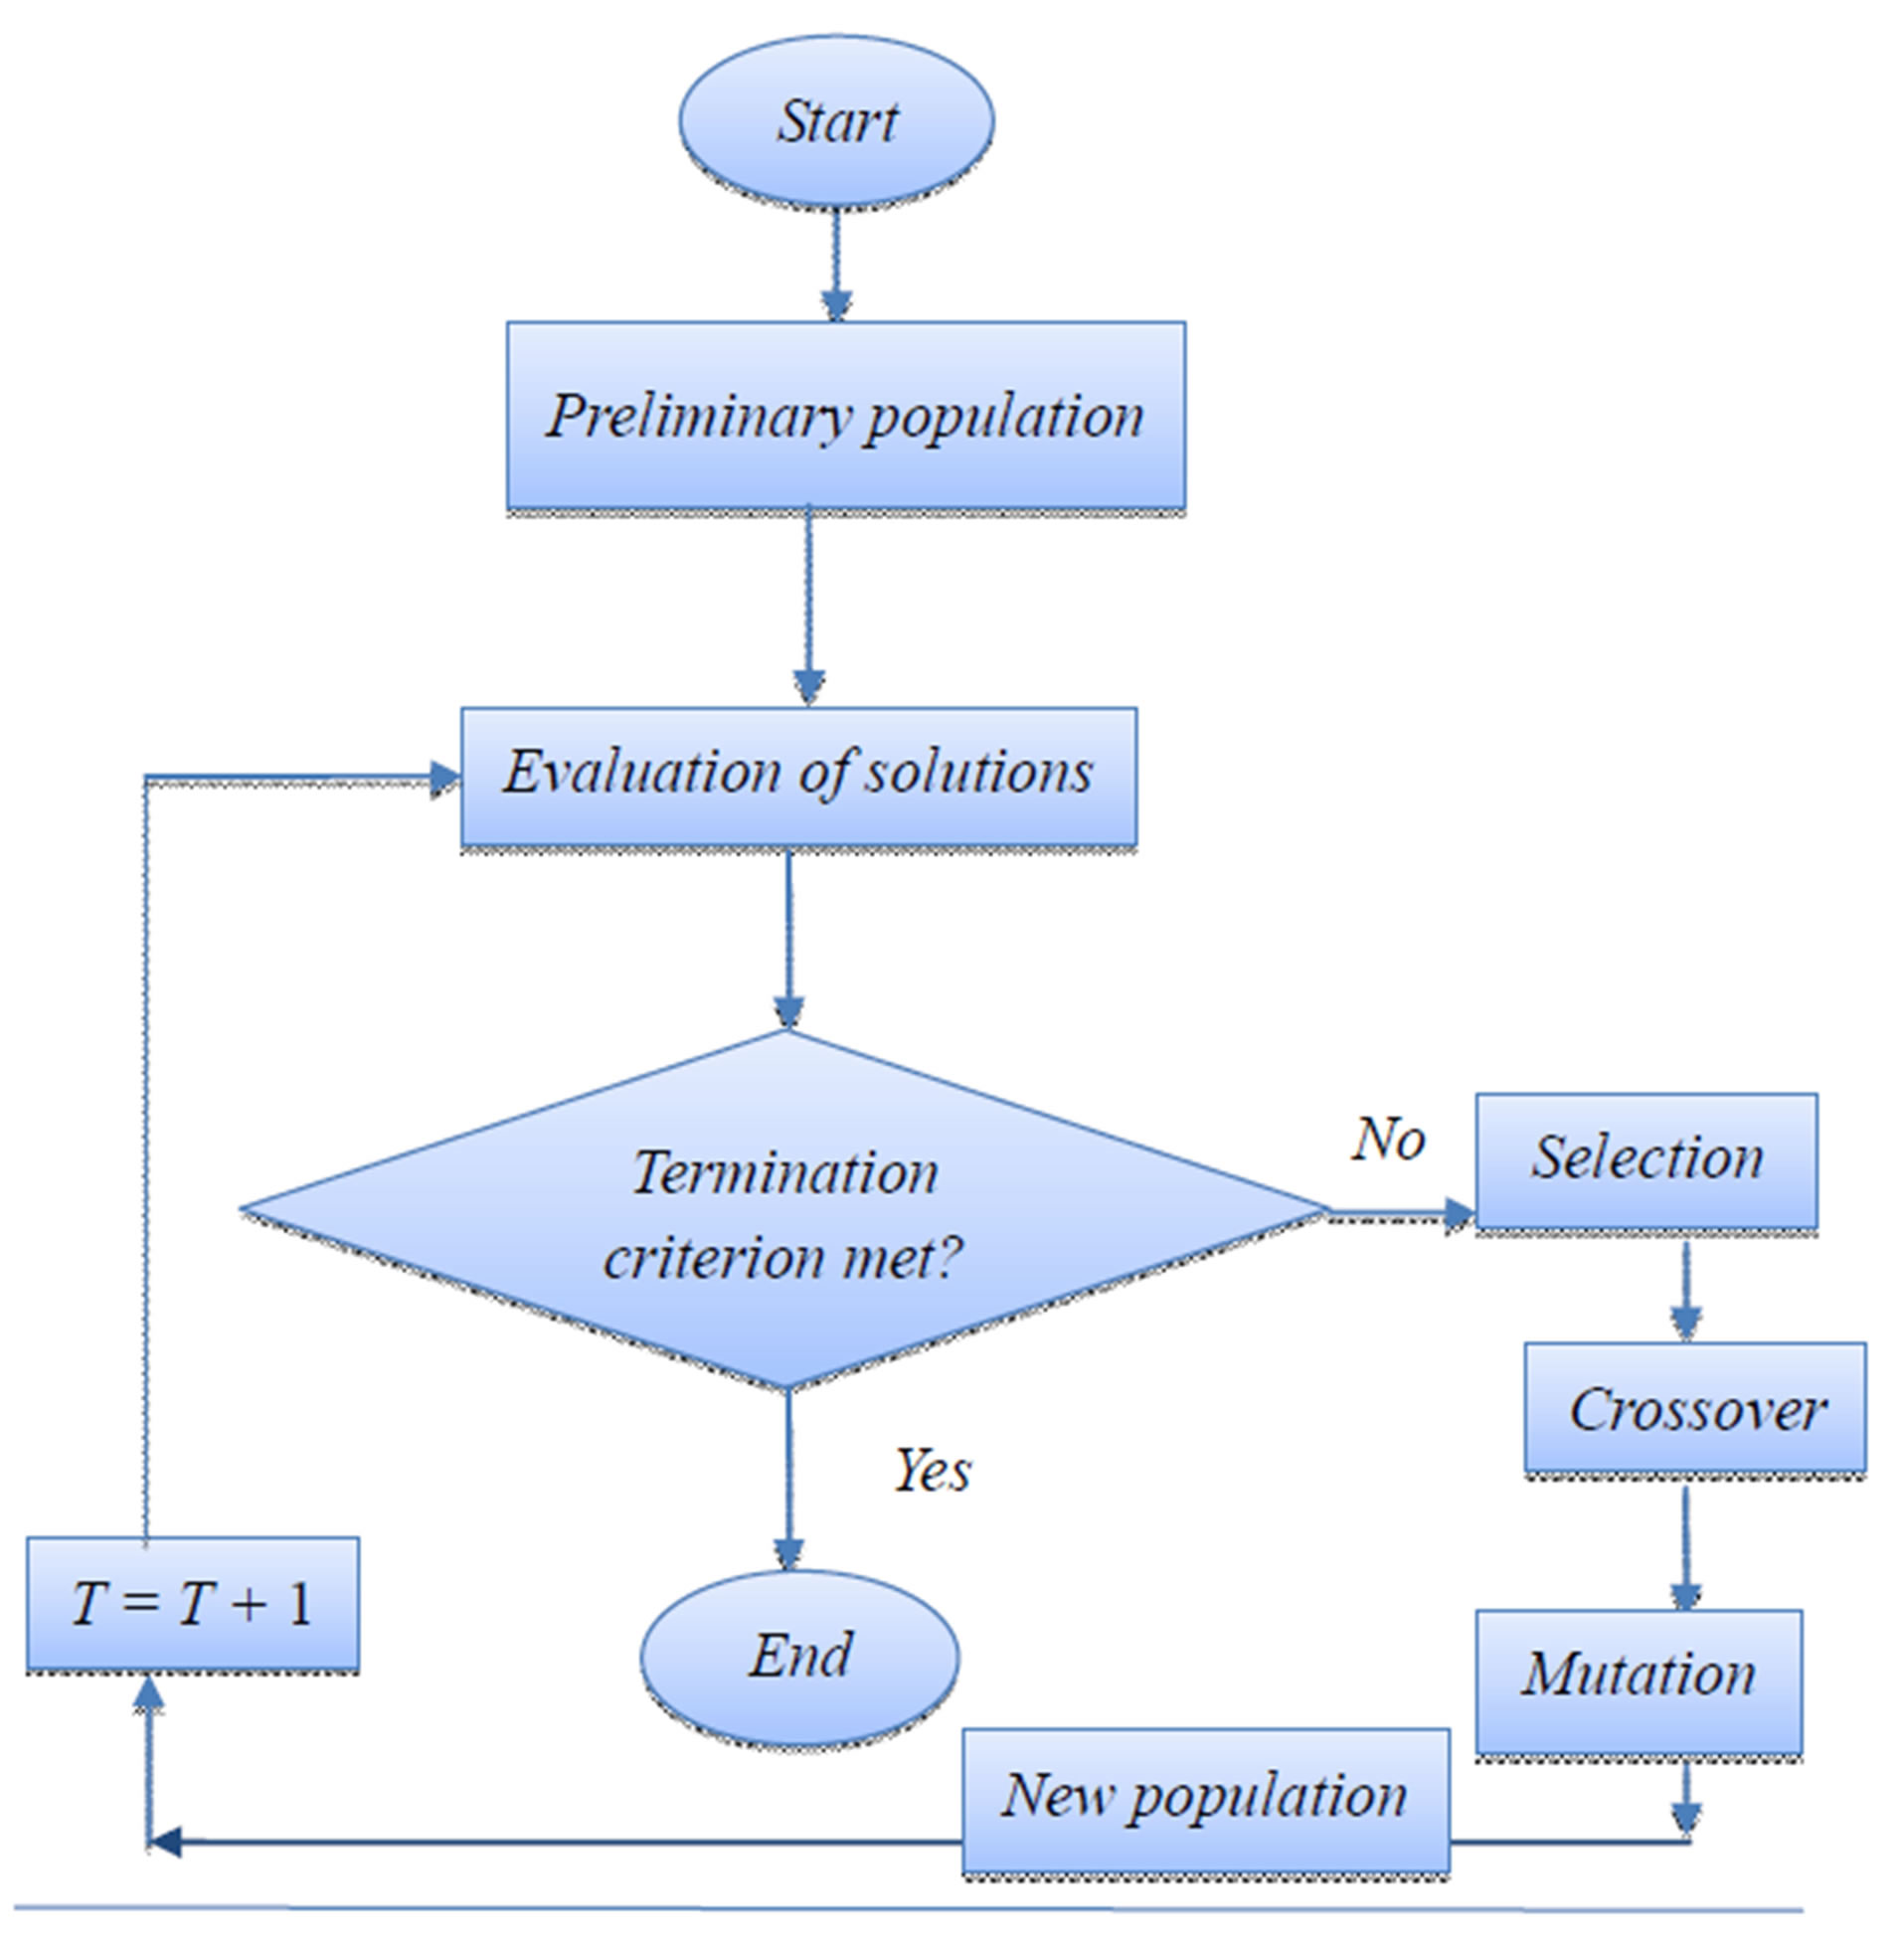
\includegraphics[width=0.6\linewidth]{figs/ga.jpg}
\\
\href{http://file.scirp.org/Html/1-8302163_41175.htm}{(Source)}
\end{center}

Once the algorithm is implemented, perform the following tasks:

\begin{enumerate}
	\item Show the best fitness found in each generation. Execute the algorithm. How does the best fitness evolve?
	\item Compare the execution time with $n=10$, $n=20$ and $n=100$. (Hint: Use the Unix command \texttt{time}).
\end{enumerate}

\end{document}
